%============================================================
% EXISTING APPROACHES
%============================================================

\section{Các phương pháp hiện có}

%============================================================
% SLIDE 1 - OVERVIEW
%============================================================

\begin{frame}
    \frametitle{Các phương pháp hiện có}

    \begin{block}{Các phương pháp hiện có sử dụng những cơ chế khác nhau
    để quyết định khi nào cần retrieval}
        Có thể phân loại dựa trên cách retrieval được quyết định
        và cách mô hình học retrieval behavior.
    \end{block}

    \vspace{0.2cm}

    \begin{center}
    \small
    \renewcommand{\arraystretch}{1.45}

    \begin{tabular}{p{2.5cm} p{2.4cm} p{2.3cm} p{5.0cm}}
        \toprule
        \textbf{Phương pháp} &
        \textbf{Cơ chế} &
        \textbf{Cách học} &
        \textbf{Retrieval Strategy} \\
        \midrule

        \textbf{IRCoT}
        &
        Heuristic
        &
        Prompting
        &
        Retrieval được thực hiện xen kẽ với
        Chain-of-Thought reasoning.
        \\[0.1cm]

        \textbf{Self-RAG}
        &
        Adaptive
        &
        Supervised
        &
        Học reflection signals để điều khiển retrieval
        và đánh giá thông tin được truy hồi.
        \\[0.1cm]

        \textbf{R-Search}
        &
        Dynamic
        &
        Reinforcement Learning
        &
        Học trajectory reasoning--search thông qua
        multi-reward reinforcement learning.
        \\

        \bottomrule
    \end{tabular}

    \end{center}

    \vspace{0.2cm}

    \begin{center}
        \textbf{\large
        Các cơ chế khác nhau dẫn đến các retrieval behavior khác nhau.
        }
    \end{center}

\end{frame}


%============================================================
% SLIDE 2 - PARAMETRIC
%============================================================

\begin{frame}
    \frametitle{Parametric Language Model}

    \begin{block}{Cách hoạt động}
        Mô hình trả lời câu hỏi chỉ dựa trên kiến thức đã được
        học và lưu trữ trong các tham số của mô hình.
    \end{block}

    \vspace{0.3cm}

    \begin{center}
    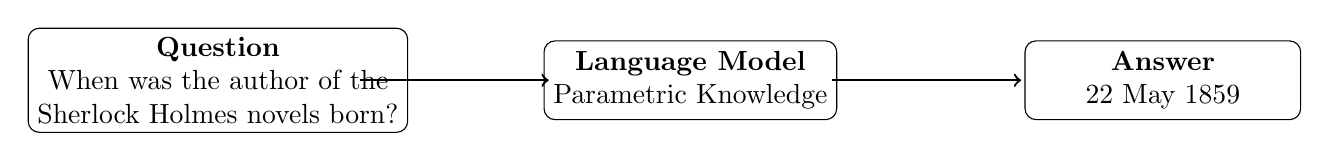
\begin{tikzpicture}[
        every node/.style={align=center},
        box/.style={
            draw,
            rounded corners,
            minimum width=3.5cm,
            minimum height=1cm
        },
        arrow/.style={
            ->,
            thick
        }
    ]

        \node[box] at (0,0)
        {\textbf{Question}\\
        When was the author of the\\
        Sherlock Holmes novels born?};

        \node[box] at (6,0)
        {\textbf{Language Model}\\
        Parametric Knowledge};

        \node[box] at (12,0)
        {\textbf{Answer}\\
        22 May 1859};

        \draw[arrow] (1.8,0) -- (4.2,0);
        \draw[arrow] (7.8,0) -- (10.2,0);

    \end{tikzpicture}
    \end{center}

    \vspace{0.3cm}

    \begin{itemize}
        \item Nếu mô hình đã học được kiến thức cần thiết,
        mô hình có thể trả lời trực tiếp.

        \item Nếu kiến thức không có hoặc không đủ trong tham số,
        mô hình có thể không biết hoặc hallucinate.

        \item Không có nguồn thông tin bên ngoài được truy hồi
        trong quá trình sinh.
    \end{itemize}

    \begin{block}{Hạn chế}
        \centering
        \textbf{Phụ thuộc hoàn toàn vào kiến thức được lưu trong
        tham số của mô hình.}
    \end{block}

\end{frame}


%============================================================
% SLIDE 3 - VANILLA RAG
%============================================================

\begin{frame}
    \frametitle{Vanilla RAG}

    \begin{block}{Cách hoạt động}
        Truy hồi thông tin một lần từ câu hỏi, sau đó đưa các
        passage được truy hồi vào mô hình để sinh câu trả lời.
    \end{block}

    \vspace{0.25cm}

    \begin{center}
    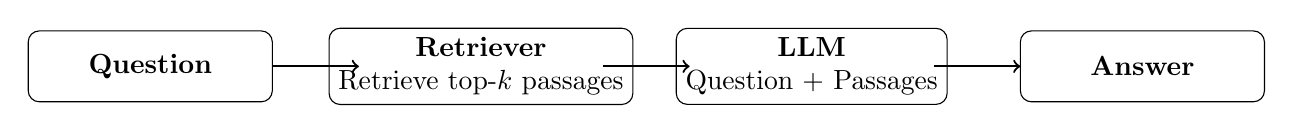
\begin{tikzpicture}[
        every node/.style={align=center},
        box/.style={
            draw,
            rounded corners,
            minimum width=3.1cm,
            minimum height=0.9cm
        },
        arrow/.style={
            ->,
            thick
        }
    ]

        \node[box] at (0,0)
        {\textbf{Question}};

        \node[box] at (4.2,0)
        {\textbf{Retriever}\\
        Retrieve top-$k$ passages};

        \node[box] at (8.4,0)
        {\textbf{LLM}\\
        Question + Passages};

        \node[box] at (12.6,0)
        {\textbf{Answer}};

        \draw[arrow] (1.55,0) -- (2.65,0);
        \draw[arrow] (5.75,0) -- (6.85,0);
        \draw[arrow] (9.95,0) -- (11.05,0);

    \end{tikzpicture}
    \end{center}

    \vspace{0.25cm}

    \begin{itemize}
        \item \textbf{Ưu điểm:}
        đơn giản, dễ triển khai và bổ sung kiến thức bên ngoài
        cho mô hình.

        \item \textbf{Hạn chế:}
        retrieval chỉ được thực hiện một lần trước khi sinh.

        \item Nếu lần retrieval đầu tiên không lấy được đầy đủ các
        passage cần thiết, mô hình không có cơ chế truy hồi bổ sung
        trong quá trình reasoning.
    \end{itemize}

    \vspace{0.05cm}

    \begin{center}
        \textbf{Một lần retrieval $\rightarrow$ một lần đọc $\rightarrow$ sinh}
    \end{center}

\end{frame}


%============================================================
% SLIDE 4 - IRCoT IMAGE
%============================================================

\begin{frame}
    \frametitle{IRCoT}

    \begin{center}
        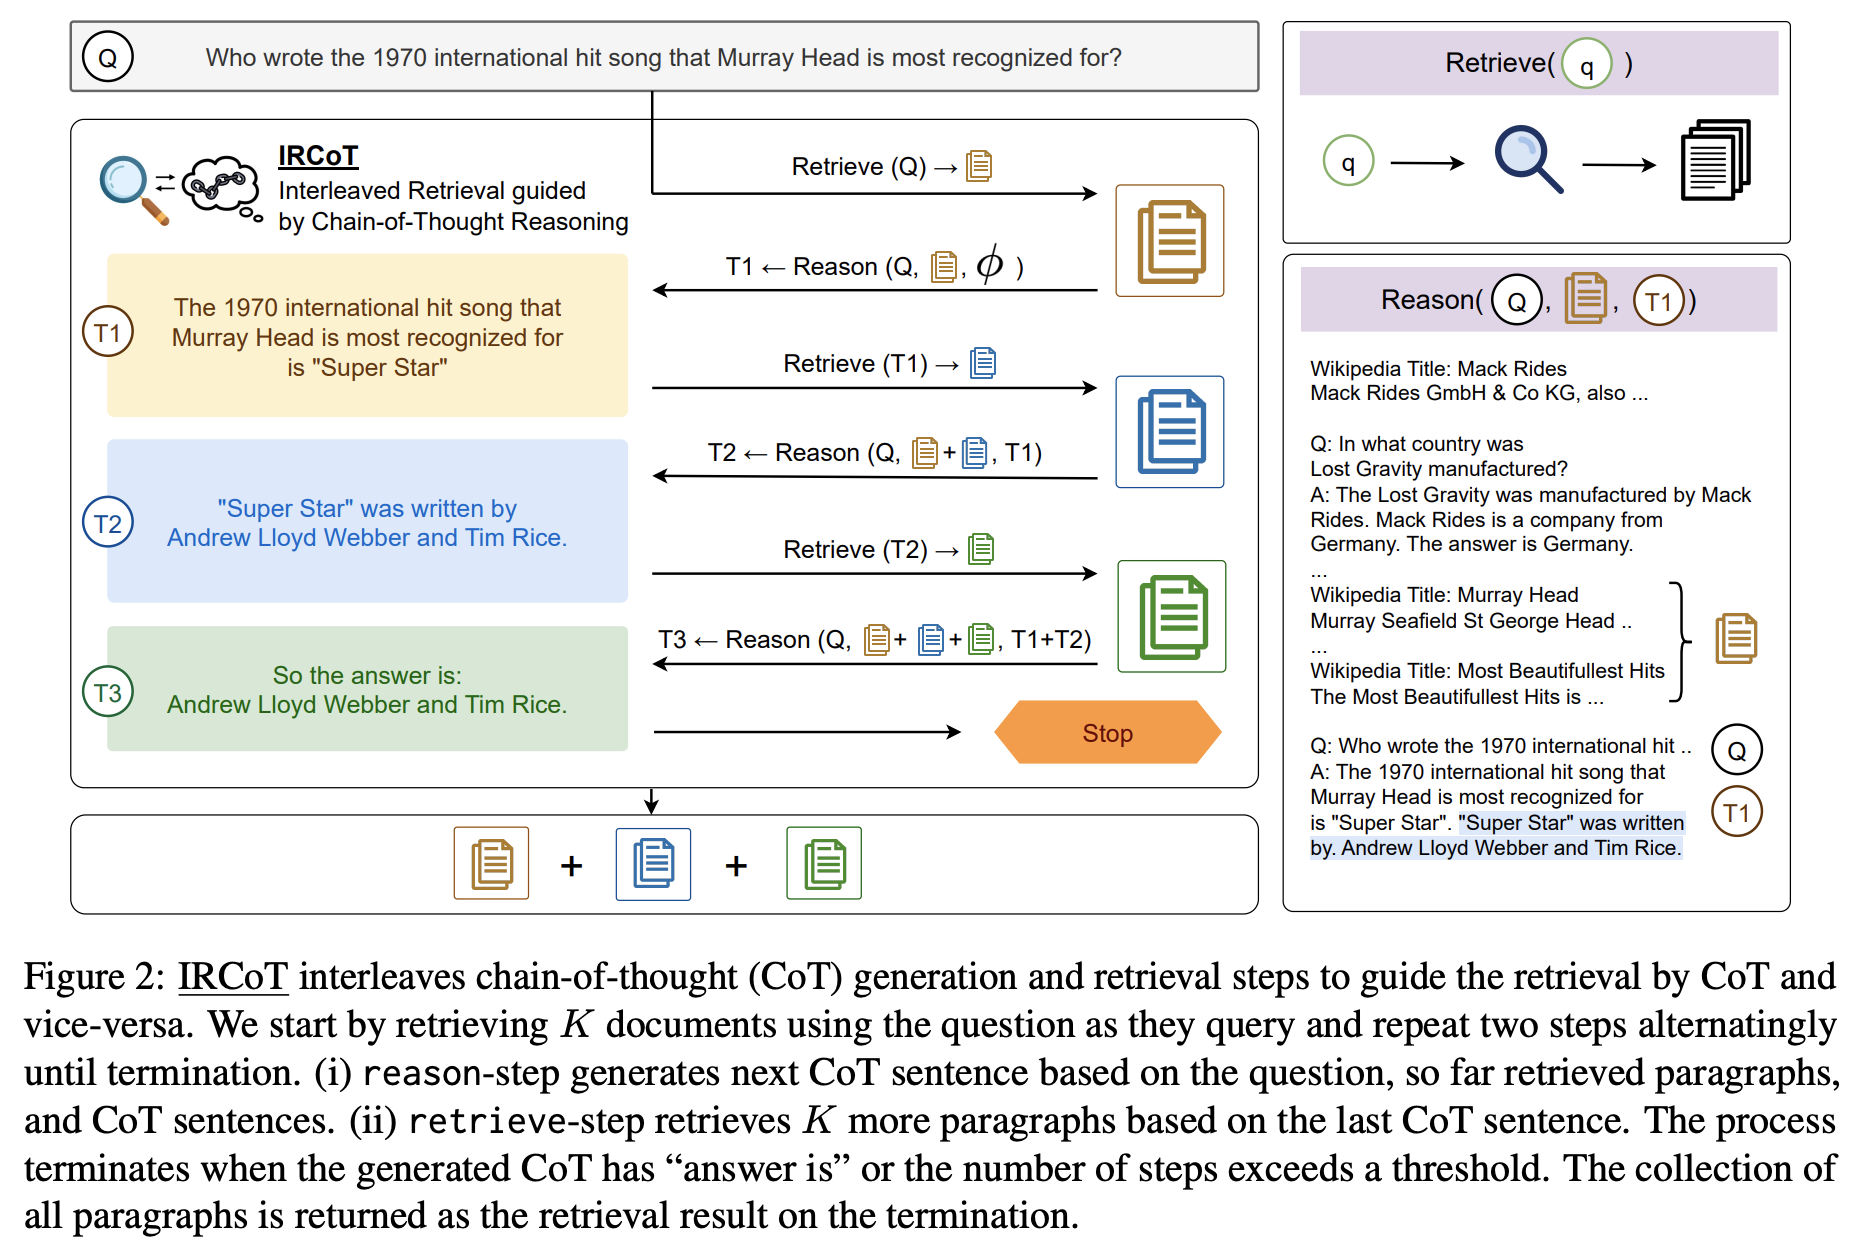
\includegraphics[
            width=0.88\textwidth,
            height=0.73\textheight,
            keepaspectratio
        ]{images/ircot.jpg}
    \end{center}

    \vspace{-0.1cm}

    \begin{center}
        \textbf{Interleave Retrieval with Chain-of-Thought Reasoning}
    \end{center}

\end{frame}


%============================================================
% SLIDE 5 - IRCoT EXAMPLE
%============================================================

\begin{frame}
    \frametitle{IRCoT: Ví dụ}

    \small

    \begin{block}{Câu hỏi}
        \textbf{When was the author of the Sherlock Holmes novels born?}
    \end{block}

    \vspace{0.1cm}

    \begin{enumerate}
        \item \textbf{Question}
        \[
        \text{Who is the author of Sherlock Holmes?}
        \]

        \item \textbf{Retrieve}
        \[
        \text{Arthur Conan Doyle}
        \]

        \item \textbf{Reason}
        \[
        \text{Arthur Conan Doyle was the author of Sherlock Holmes.}
        \]

        \item \textbf{Retrieve}
        \[
        \text{Arthur Conan Doyle was born on 22 May 1859.}
        \]

        \item \textbf{Answer}
        \[
        \boxed{\text{22 May 1859}}
        \]
    \end{enumerate}

    \vspace{0.02cm}

    \begin{block}{Cơ chế}
        Retrieval được thực hiện xen kẽ với các bước reasoning.
        Kết quả reasoning ở bước trước được sử dụng để tạo truy vấn
        retrieval tiếp theo.
    \end{block}

\end{frame}


%============================================================
% SLIDE 6 - IRCoT DETAILS
%============================================================

\begin{frame}
    \frametitle{IRCoT: Cơ chế, ưu điểm và hạn chế}

    \small

    \begin{block}{Cơ chế}
        IRCoT interleave Chain-of-Thought reasoning với retrieval:
        các bước reasoning trung gian được sử dụng để tạo các
        truy vấn retrieval tiếp theo.
    \end{block}

    \vspace{0.15cm}

    \begin{itemize}
        \setlength{\itemsep}{4pt}

        \item \textbf{Retrieval mechanism:}
        sử dụng BM25 thông qua Elasticsearch; các truy vấn tiếp theo
        sử dụng câu đầu tiên của CoT hiện tại.

        \item \textbf{Cách học:}
        inference-time few-shot prompting, không có
        retrieval-decision training riêng.

        \item \textbf{Ưu điểm:}
        reasoning trung gian giúp retrieval được thông tin cần thiết
        cho các câu hỏi multi-hop.

        \item \textbf{Hạn chế:}
        retrieval phụ thuộc chặt vào reasoning process, do đó có thể
        trigger retrieval ngay cả khi không cần thông tin bên ngoài,
        làm tăng retrieval cost.

    \end{itemize}

    \vspace{0.1cm}

    \begin{block}{Vấn đề}
        \centering
        \textbf{Retrieval được điều khiển bởi reasoning procedure,
        thay vì một quyết định riêng về việc có cần retrieval hay không.}
    \end{block}

    \vspace{0.02cm}

    \begin{center}
        \scriptsize
        Trivedi et al., \textit{IRCoT}, ACL 2023
    \end{center}

\end{frame}


%============================================================
% SLIDE 7 - SELF-RAG IMAGE
%============================================================

\begin{frame}
    \frametitle{Self-RAG}

    \begin{center}
        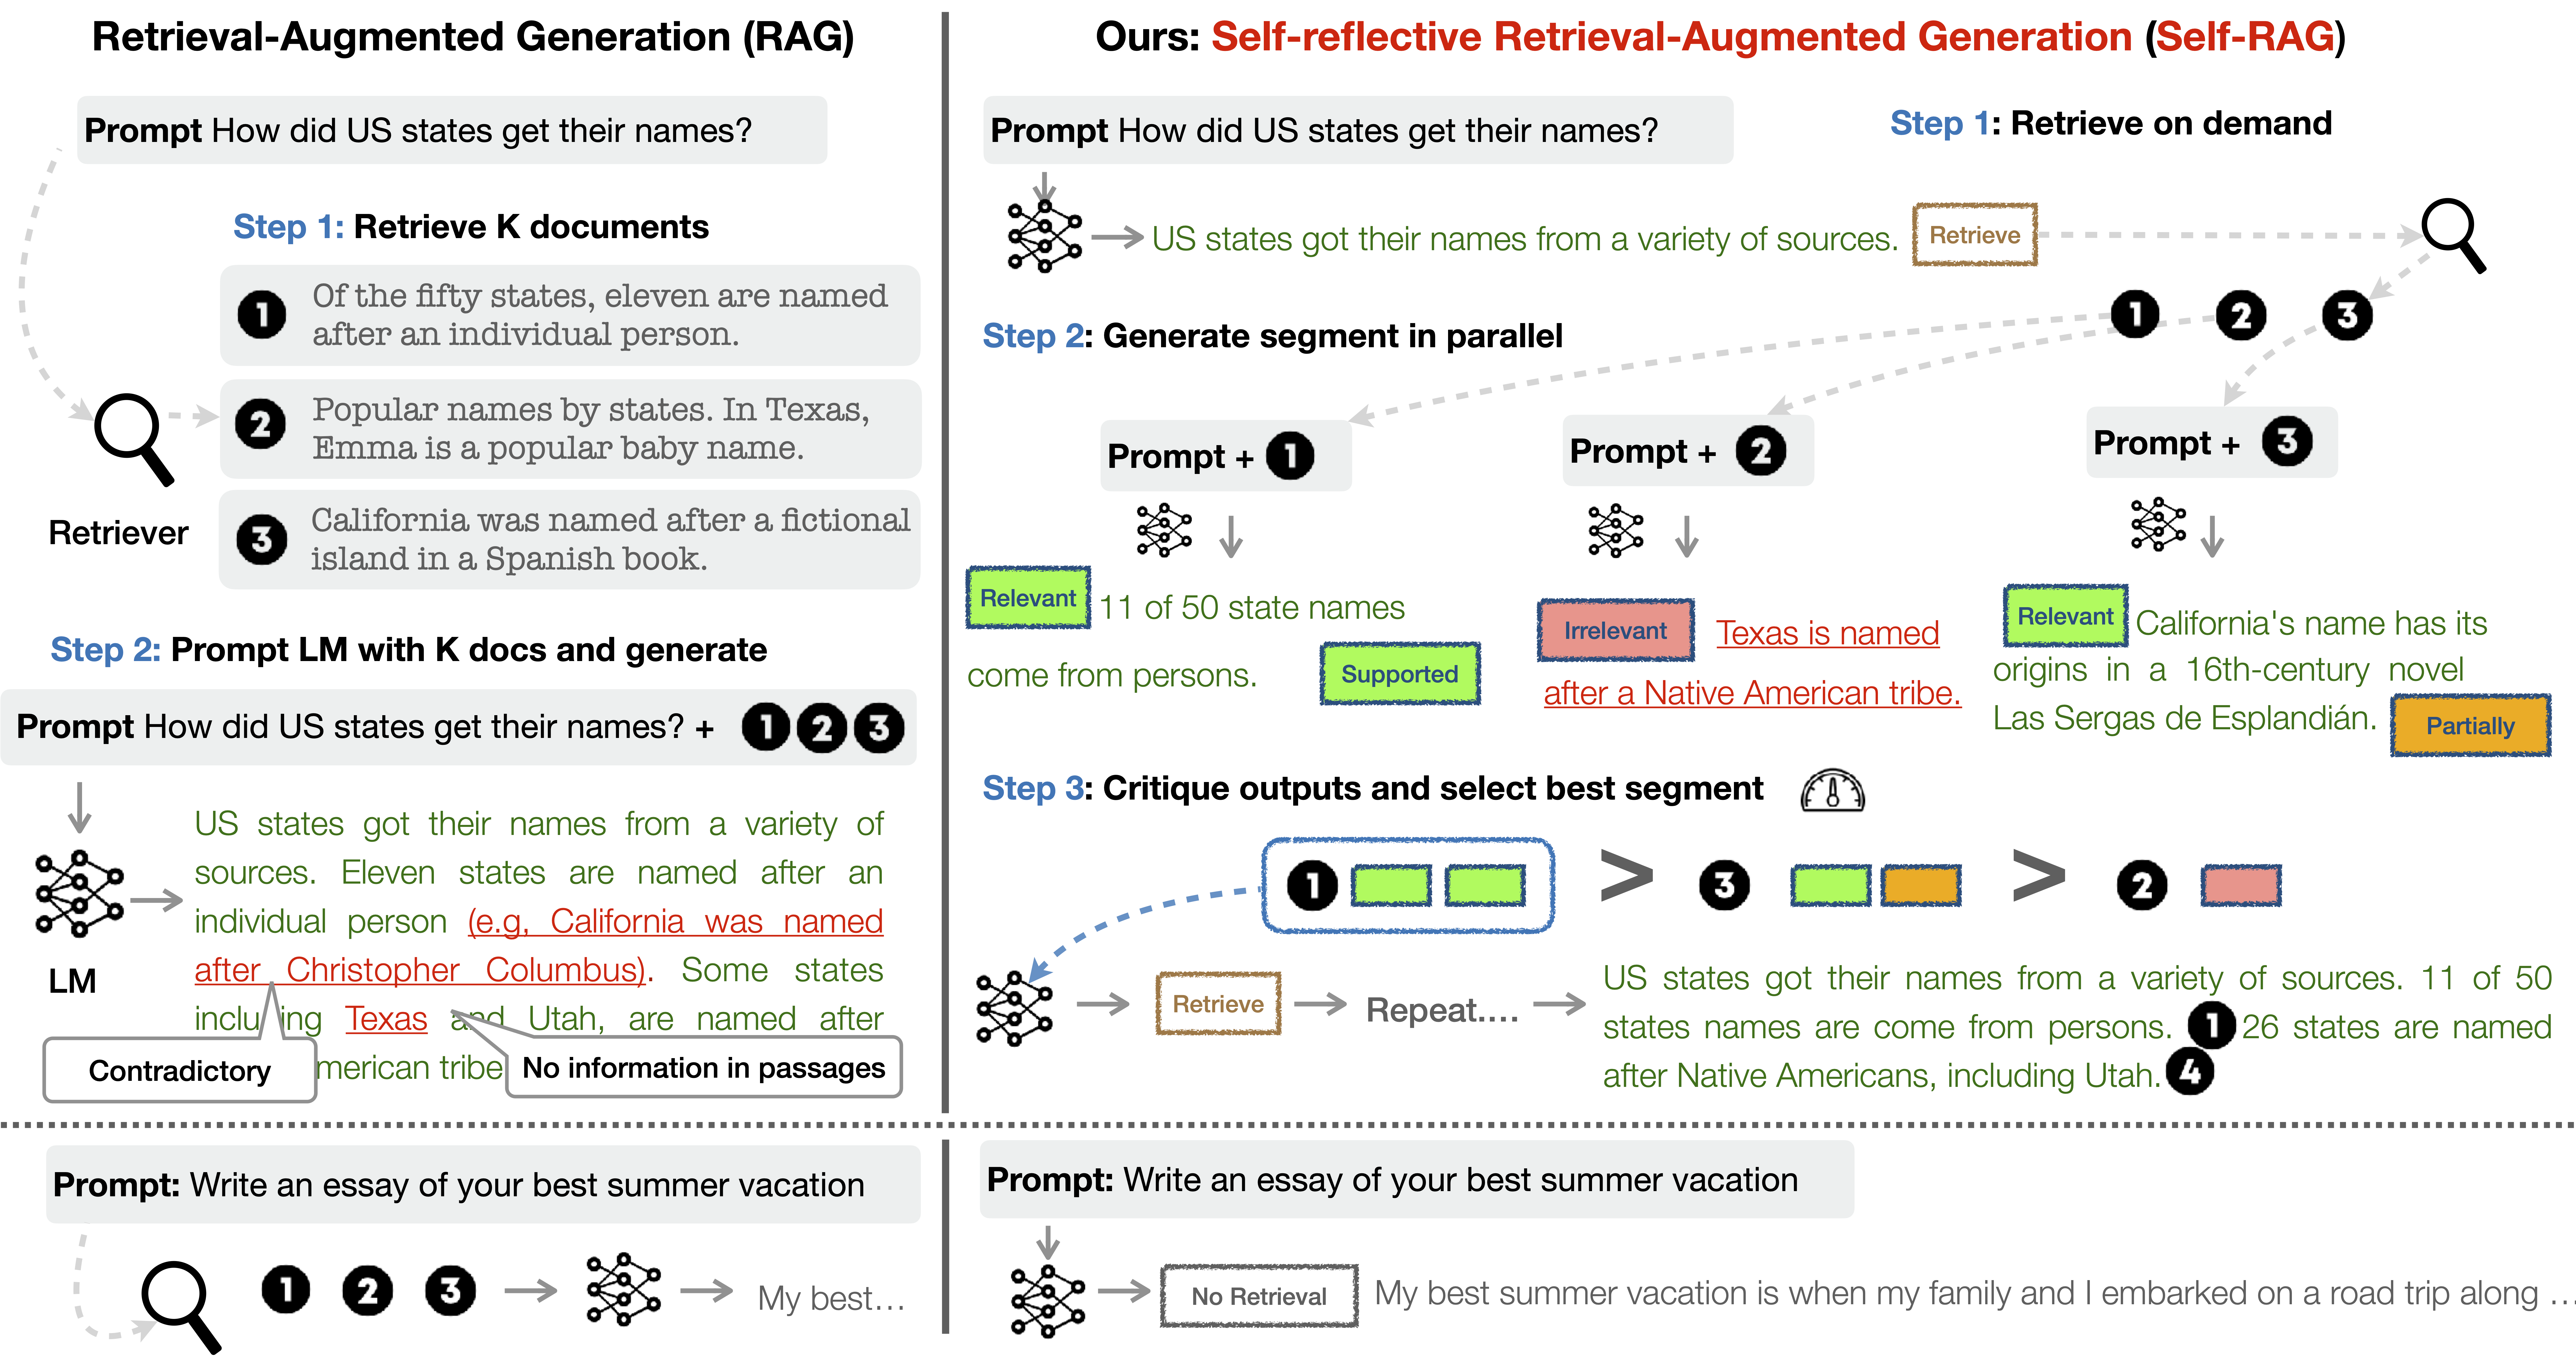
\includegraphics[
            width=0.88\textwidth,
            height=0.73\textheight,
            keepaspectratio
        ]{images/self_rag.png}
    \end{center}

    \vspace{-0.1cm}

    \begin{center}
        \textbf{Adaptive Retrieval with Self-Reflection}
    \end{center}

\end{frame}


%============================================================
% SLIDE 8 - SELF-RAG EXAMPLE
%============================================================

\begin{frame}
    \frametitle{Self-RAG: Ví dụ}

    \small

    \begin{block}{Câu hỏi}
        \textbf{When was the author of the Sherlock Holmes novels born?}
    \end{block}

    \vspace{0.1cm}

    \begin{center}
    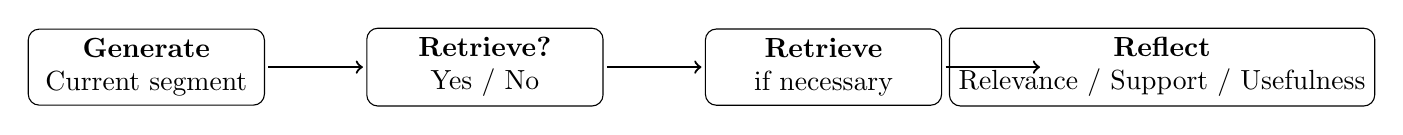
\begin{tikzpicture}[
        every node/.style={align=center},
        box/.style={
            draw,
            rounded corners,
            minimum width=3.0cm,
            minimum height=0.85cm
        },
        arrow/.style={
            ->,
            thick
        }
    ]

        \node[box] at (0,0)
        {\textbf{Generate}\\
        Current segment};

        \node[box] at (4.3,0)
        {\textbf{Retrieve?}\\
        Yes / No};

        \node[box] at (8.6,0)
        {\textbf{Retrieve}\\
        if necessary};

        \node[box] at (12.9,0)
        {\textbf{Reflect}\\
        Relevance / Support / Usefulness};

        \draw[arrow] (1.55,0) -- (2.75,0);
        \draw[arrow] (5.85,0) -- (7.05,0);
        \draw[arrow] (10.15,0) -- (11.35,0);

    \end{tikzpicture}
    \end{center}

    \vspace{0.2cm}

    \begin{itemize}
        \item Mô hình có thể quyết định có cần retrieval hay không.

        \item Nếu cần, mô hình gọi retriever và sử dụng
        passage được truy hồi để tiếp tục sinh.

        \item Reflection tokens được sử dụng để kiểm soát retrieval
        và đánh giá thông tin được truy hồi.
    \end{itemize}

\end{frame}


%============================================================
% SLIDE 9 - SELF-RAG DETAILS
%============================================================

\begin{frame}
    \frametitle{Self-RAG: Cơ chế, ưu điểm và hạn chế}

    \small

    \begin{block}{Cơ chế}
        Train một LM để quyết định khi nào cần retrieval trong quá
        trình generation và tự phản ánh về thông tin được truy hồi.
    \end{block}

    \vspace{0.15cm}

    \begin{itemize}
        \setlength{\itemsep}{4pt}

        \item \textbf{Adaptive retrieval:}
        mô hình quyết định có cần retrieval trong quá trình sinh.

        \item \textbf{Reflection tokens:}
        các token đặc biệt được sử dụng để điều khiển retrieval
        và đánh giá retrieved evidence.

        \item \textbf{Cách học:}
        retrieval decisions được học thông qua
        supervised reflection tokens.

        \item \textbf{Ưu điểm:}
        retrieval trở thành một phần thích ứng của generation,
        thay vì là một bước preprocessing cố định.

        \item \textbf{Hạn chế:}
        cần xây dựng supervision cho retrieval decisions và
        reflection tokens.

    \end{itemize}

    \vspace{0.08cm}

    \begin{block}{Điểm khác biệt}
        \centering
        \textbf{Self-RAG học trực tiếp retrieval behavior thông qua
        supervised reflection signals.}
    \end{block}

    \vspace{0.02cm}

    \begin{center}
        \scriptsize
        Asai et al., \textit{Self-RAG}, ICLR 2024
    \end{center}

\end{frame}


%============================================================
% SLIDE 10 - SELF-RAG TRAINING
%============================================================

\begin{frame}
    \frametitle{Self-RAG: Supervised Retrieval Decisions}

    \small

    \begin{block}{Training paradigm}
        Self-RAG học retrieval decisions thông qua
        supervised reflection tokens.
    \end{block}

    \vspace{0.1cm}

    \begin{center}
    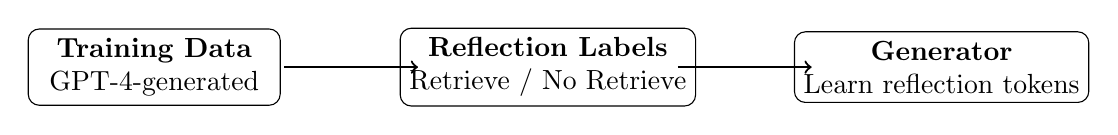
\begin{tikzpicture}[
        every node/.style={align=center},
        box/.style={
            draw,
            rounded corners,
            minimum width=3.2cm,
            minimum height=0.8cm
        },
        arrow/.style={
            ->,
            thick
        }
    ]

        \node[box] at (0,0)
        {\textbf{Training Data}\\
        GPT-4-generated};

        \node[box] at (5,0)
        {\textbf{Reflection Labels}\\
        Retrieve / No Retrieve};

        \node[box] at (10,0)
        {\textbf{Generator}\\
        Learn reflection tokens};

        \draw[arrow] (1.65,0) -- (3.35,0);
        \draw[arrow] (6.65,0) -- (8.35,0);

    \end{tikzpicture}
    \end{center}

    \vspace{0.12cm}

    \begin{itemize}
        \setlength{\itemsep}{3pt}

        \item \textbf{Explicit supervision:}
        retrieval decisions được biểu diễn trực tiếp bởi
        reflection-token labels.

        \item \textbf{Label dependency:}
        training cần xây dựng supervision chất lượng cao
        cho retrieval decisions.

        \item \textbf{Domain/task dependency:}
        supervised RAG methods có thể cần adaptation khi
        chuyển sang domain hoặc task chuyên biệt.

    \end{itemize}

    \vspace{0.05cm}

    \begin{center}
        \scriptsize
        Asai et al., \textit{Self-RAG}, ICLR 2024
        \quad
        Mao et al., \textit{RAG-Studio}, Findings EMNLP 2024
    \end{center}

\end{frame}


%============================================================
% SLIDE 11 - R-SEARCH IMAGE
%============================================================

\begin{frame}
    \frametitle{R-Search}

    \begin{center}
        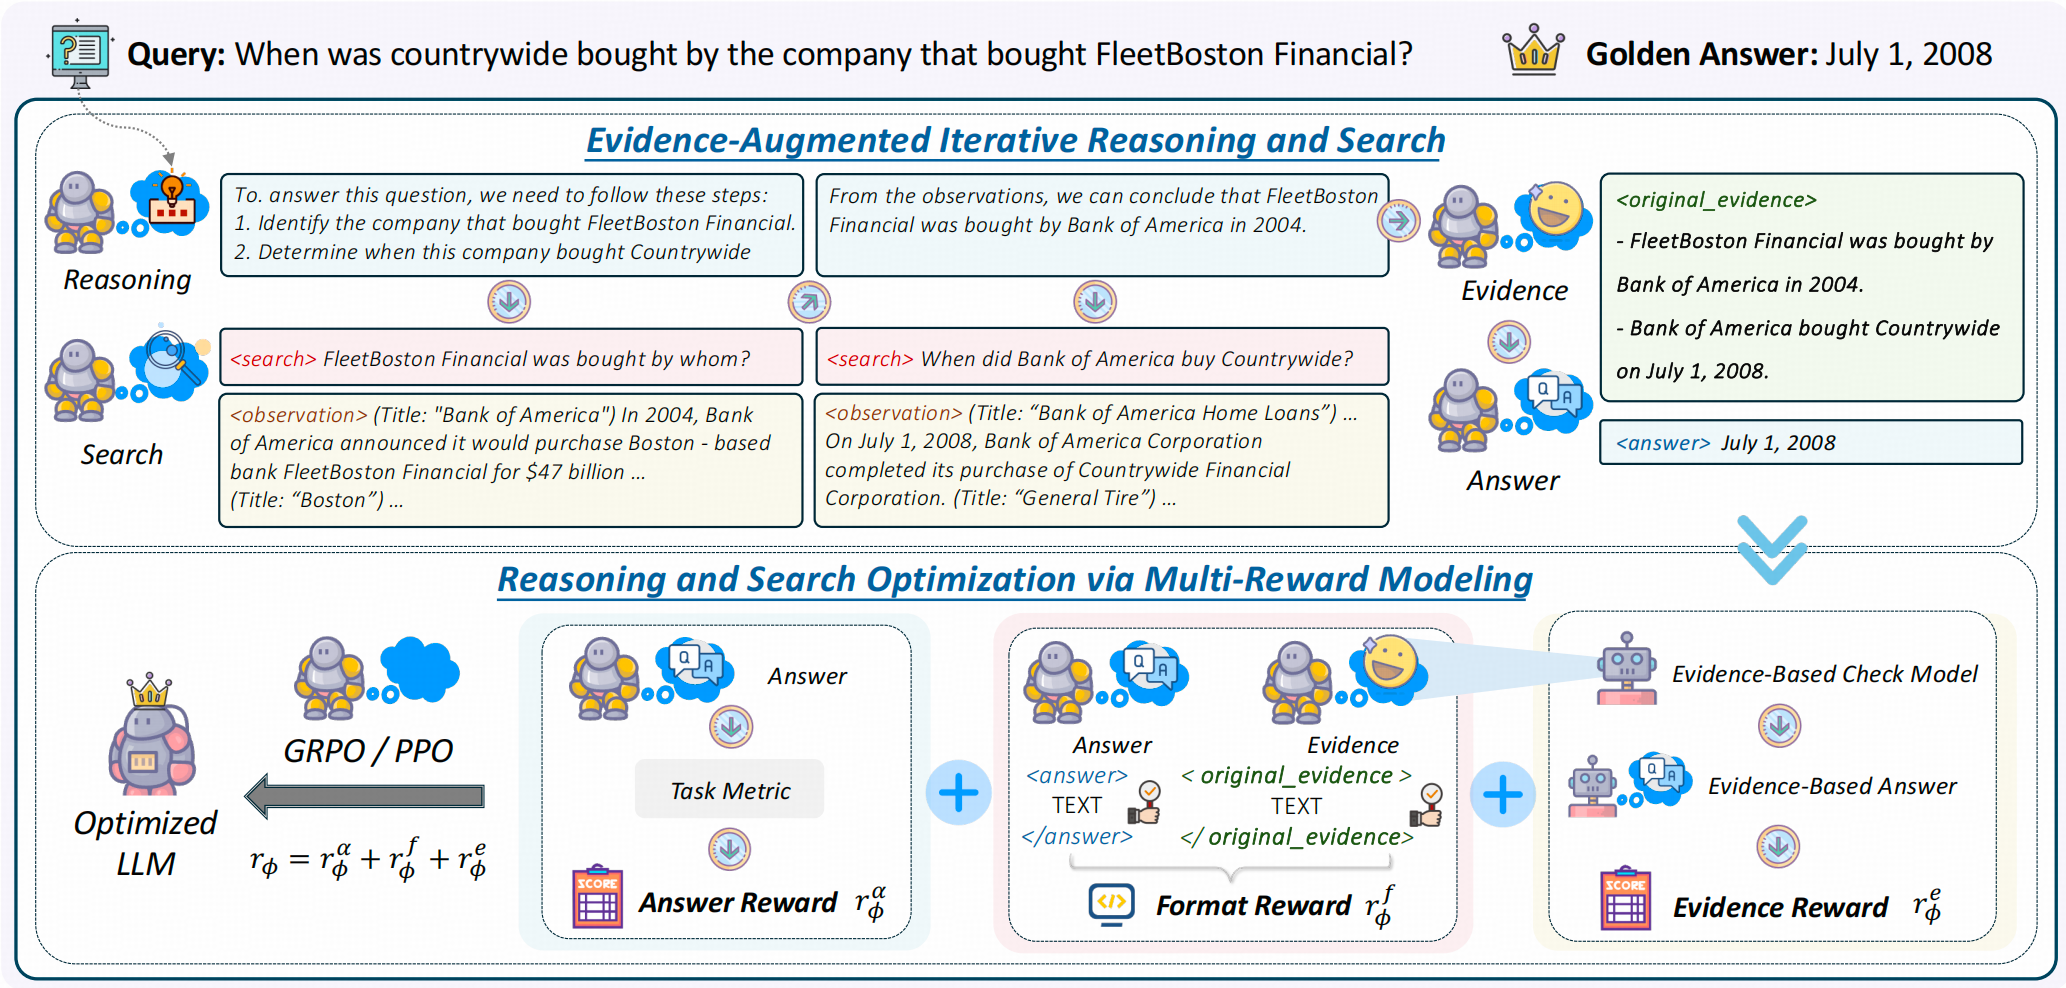
\includegraphics[
            width=0.88\textwidth,
            height=0.73\textheight,
            keepaspectratio
        ]{images/rsearch.png}
    \end{center}

    \vspace{-0.1cm}

    \begin{center}
        \textbf{Reasoning--Search Integration with Reinforcement Learning}
    \end{center}

\end{frame}


%============================================================
% SLIDE 12 - R-SEARCH EXAMPLE
%============================================================

\begin{frame}
    \frametitle{R-Search: Ví dụ}

    \small

    \begin{block}{Câu hỏi}
        \textbf{When was the author of the Sherlock Holmes novels born?}
    \end{block}

    \vspace{0.1cm}

    \begin{center}
    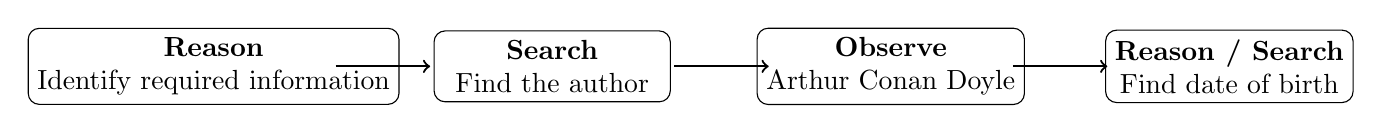
\begin{tikzpicture}[
        every node/.style={align=center},
        box/.style={
            draw,
            rounded corners,
            minimum width=3.0cm,
            minimum height=0.85cm
        },
        arrow/.style={
            ->,
            thick
        }
    ]

        \node[box] at (0,0)
        {\textbf{Reason}\\
        Identify required information};

        \node[box] at (4.3,0)
        {\textbf{Search}\\
        Find the author};

        \node[box] at (8.6,0)
        {\textbf{Observe}\\
        Arthur Conan Doyle};

        \node[box] at (12.9,0)
        {\textbf{Reason / Search}\\
        Find date of birth};

        \draw[arrow] (1.55,0) -- (2.75,0);
        \draw[arrow] (5.85,0) -- (7.05,0);
        \draw[arrow] (10.15,0) -- (11.35,0);

    \end{tikzpicture}
    \end{center}

    \vspace{0.2cm}

    \begin{block}{Cơ chế}
        Mô hình học cách tương tác giữa reasoning và search:
        quyết định khi nào reasoning tiếp tục và khi nào cần search
        thông qua reinforcement learning.
    \end{block}

\end{frame}


%============================================================
% SLIDE 13 - R-SEARCH DETAILS
%============================================================

\begin{frame}
    \frametitle{R-Search: Cơ chế, ưu điểm và hạn chế}

    \small

    \begin{block}{Cơ chế}
        Sử dụng reinforcement learning để học cách LLM
        dynamically interleave reasoning và search.
    \end{block}

    \vspace{0.15cm}

    \begin{itemize}
        \setlength{\itemsep}{4pt}

        \item \textbf{Dynamic search:}
        policy quyết định khi nào search trong quá trình generation
        bằng cách tạo các search actions.

        \item \textbf{Multi-step interaction:}
        search và reasoning có thể được thực hiện xen kẽ nhiều lần
        trong cùng một trajectory.

        \item \textbf{Evidence synthesis:}
        thông tin được truy hồi được tổng hợp trước khi
        tạo câu trả lời cuối cùng.

        \item \textbf{Ưu điểm:}
        không cần explicit retrieval-decision labels;
        search behavior được học từ trajectory-level rewards.

        \item \textbf{Hạn chế:}
        reinforcement learning yêu cầu repeated rollout,
        search, reward computation và policy updates,
        dẫn đến chi phí tính toán đáng kể.

        \item \textbf{Hạn chế:}
        retrieval timing được tối ưu gián tiếp như một phần của
        reasoning--search trajectory.

    \end{itemize}

    \vspace{0.05cm}

    \begin{block}{Điểm khác biệt}
        \centering
        \textbf{R-Search học retrieval behavior thông qua
        trajectory-level reinforcement learning.}
    \end{block}

    \vspace{0.02cm}

    \begin{center}
        \scriptsize
        Zhao et al., \textit{R-Search}, Findings of ACL 2026
    \end{center}

\end{frame}


%============================================================
% SLIDE 14 - R-SEARCH TRAINING
%============================================================

\begin{frame}
    \frametitle{R-Search: Multi-Reward Reinforcement Learning}

    \small

    \begin{block}{Training paradigm}
        R-Search tối ưu reasoning--search trajectories
        sử dụng nhiều reward signals với reinforcement learning.
    \end{block}

    \vspace{0.12cm}

    \begin{center}
    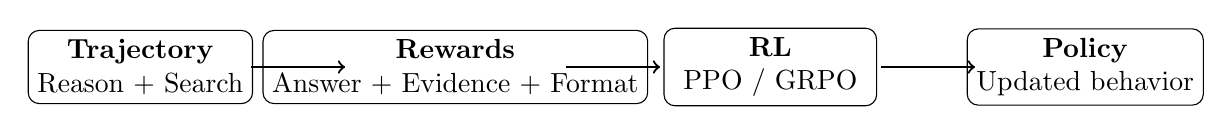
\begin{tikzpicture}[
        every node/.style={align=center},
        box/.style={
            draw,
            rounded corners,
            minimum width=2.7cm,
            minimum height=0.78cm
        },
        arrow/.style={
            ->,
            thick
        }
    ]

        \node[box] at (0,0)
        {\textbf{Trajectory}\\
        Reason + Search};

        \node[box] at (4,0)
        {\textbf{Rewards}\\
        Answer + Evidence + Format};

        \node[box] at (8,0)
        {\textbf{RL}\\
        PPO / GRPO};

        \node[box] at (12,0)
        {\textbf{Policy}\\
        Updated behavior};

        \draw[arrow] (1.4,0) -- (2.6,0);
        \draw[arrow] (5.4,0) -- (6.6,0);
        \draw[arrow] (9.4,0) -- (10.6,0);

    \end{tikzpicture}
    \end{center}

    \vspace{0.12cm}

    \begin{itemize}
        \setlength{\itemsep}{3pt}

        \item \textbf{Không cần retrieval-decision labels:}
        search behavior được học từ trajectory-level rewards.

        \item \textbf{Chi phí RL:}
        repeated rollout, search, reward computation và
        policy updates tạo thêm computational overhead.

        \item \textbf{Retrieval timing được học gián tiếp:}
        retrieval decisions được tối ưu như một phần của
        overall reasoning--search trajectory.

    \end{itemize}

    \vspace{0.08cm}

    \begin{block}{Hạn chế}
        \centering
        \textbf{Retrieval timing được học gián tiếp thông qua
        trajectory-level reinforcement learning.}
    \end{block}

    \vspace{0.02cm}

    \begin{center}
        \scriptsize
        Zhao et al., \textit{R-Search}, Findings of ACL 2026
    \end{center}

\end{frame}


%============================================================
% SLIDE 15 - COMPARISON
%============================================================

\begin{frame}
    \frametitle{So sánh các phương pháp}

    \small

    \begin{center}
    \renewcommand{\arraystretch}{1.4}

    \begin{tabular}{p{2.3cm} p{2.2cm} p{2.3cm} p{5.2cm}}
        \toprule
        \textbf{Phương pháp} &
        \textbf{Retrieval} &
        \textbf{Cách học} &
        \textbf{Đặc điểm chính} \\
        \midrule

        Parametric LM
        &
        Không
        &
        Pre-training
        &
        Phụ thuộc vào kiến thức trong tham số.
        \\

        Vanilla RAG
        &
        Một lần
        &
        Không học timing
        &
        Retrieval cố định trước generation.
        \\

        IRCoT
        &
        Xen kẽ CoT
        &
        Prompting
        &
        Retrieval được điều khiển bởi các bước reasoning.
        \\

        Self-RAG
        &
        Adaptive
        &
        Supervised
        &
        Học retrieval và reflection thông qua
        reflection tokens.
        \\

        R-Search
        &
        Dynamic
        &
        RL
        &
        Học trajectory reasoning--search bằng
        multi-reward reinforcement learning.
        \\

        \bottomrule
    \end{tabular}
    \end{center}

\end{frame}


%============================================================
% SLIDE 16 - RESEARCH GAP
%============================================================

\begin{frame}
    \frametitle{Khoảng trống nghiên cứu}

    \begin{center}
    \large
    \textbf{Các phương pháp hiện có sử dụng những cơ chế khác nhau
    để điều khiển retrieval.}
    \end{center}

    \vspace{0.4cm}

    \begin{itemize}

        \item \textbf{Parametric LM:}
        không sử dụng retrieval.

        \vspace{0.1cm}

        \item \textbf{Vanilla RAG:}
        retrieval cố định một lần.

        \vspace{0.1cm}

        \item \textbf{IRCoT:}
        retrieval được điều khiển bởi quá trình reasoning.

        \vspace{0.1cm}

        \item \textbf{Self-RAG:}
        retrieval decision được học thông qua supervision
        và reflection tokens.

        \vspace{0.1cm}

        \item \textbf{R-Search:}
        retrieval behavior được học thông qua reinforcement learning.

    \end{itemize}

    \vspace{0.25cm}

    \begin{block}{Hướng tiếp cận}
        \centering
        \textbf{Học thời điểm truy hồi mà không cần
        trực tiếp giám sát decision và không sử dụng RL.}
    \end{block}

\end{frame}


%============================================================
% SLIDE 17 - RESEARCH QUESTION
%============================================================

\begin{frame}
    \frametitle{Research Question}

    \small

    \begin{block}{Từ các phương pháp hiện có}
        Các phương pháp hiện có sử dụng heuristic,
        explicit supervision hoặc reinforcement learning
        để học adaptive retrieval behavior.
    \end{block}

    \vspace{0.25cm}

    \begin{center}
        \large
        \textbf{Liệu retrieval timing có thể được học thông qua}\\
        \textbf{một cơ chế học trực tiếp và cục bộ hơn,}\\
        \textbf{mà vẫn duy trì khả năng retrieval thích ứng?}
    \end{center}

    \vspace{0.25cm}

    \begin{center}
    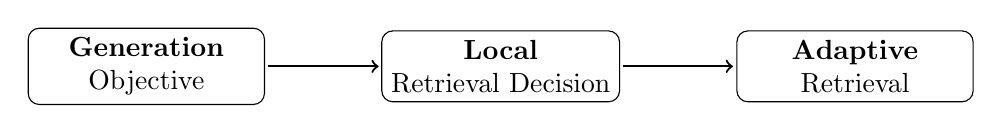
\begin{tikzpicture}[
        every node/.style={align=center},
        box/.style={
            draw,
            rounded corners,
            minimum width=3.0cm,
            minimum height=0.8cm
        },
        arrow/.style={
            ->,
            thick
        }
    ]

        \node[box] at (0,0)
        {\textbf{Generation}\\
        Objective};

        \node[box] at (4.5,0)
        {\textbf{Local}\\
        Retrieval Decision};

        \node[box] at (9,0)
        {\textbf{Adaptive}\\
        Retrieval};

        \draw[arrow] (1.55,0) -- (2.95,0);
        \draw[arrow] (6.05,0) -- (7.45,0);

    \end{tikzpicture}
    \end{center}

\end{frame}